\documentclass[conference]{IEEEtran}

\usepackage{graphicx}
\usepackage{amssymb}

\begin{document}
\title{Non-Photorealistic rendering using edge aware filters}
\author{Parla Surendra Mani kumar\\Nadiminti Praveen \\ Jagarlamudi Sai Laxman}
\maketitle

\begin{abstract}
	Our project aims to create a cartoon effect to the given input image. This was achieved using edge aware filters.	
\end{abstract}

\begin{IEEEkeywords}
	NPR, Bilater filter, image abstraction,domain transfer
\end{IEEEkeywords}

\section{introduction} \label{s1}
 Non-photorealistic rendering (NPR) is an area of computer graphics in which an image is modified to create attractive digital art and effects. The input to a two dimensional NPR system is typically an image or video. The output is a typically an artistic rendering of that input imagery (for example in a watercolor, painterly or sketched style).In our project we wish to accomplish this by using edge aware filters. Edge aware filters blurs the image without effecting the edges. 
  
 \section{General Idea}
 The general idea of how it is implemented is as follows:
 \begin{enumerate}
 \item The given image is converted from rgb to lab colour space
 \item L channel of the image is smothened using an edge aware filter
 \item The smothened L channel is then quantized to different levels and an image I1 is created, as a cartoon has few colours.
 \item The smothened L-channel is passed through an edge detection filter for detecting edges and an image I2 is created, as a cartoon highlights edges.
 \item The images I1 and I2 are combined to form modified L-channel.
 \item The modified L-channel and unmodified a,b channel is used to created our required rgb image.
 \end{enumerate}
  Figure \ref{fig:Idea} represents the basic idea of cartoonization.
  
\begin{figure}
 	\includegraphics[width = \linewidth]{Idea.jpg}
 	\caption{Idea of Cartoonization}
 	\label{fig:Idea}
 \end{figure}
 
 \section{Domain Transform}
For any1D signal we can use a transform f such that the original distances between the points are preserved. I.e,.
$$\mid f(x_i,I(x_i))-f(x_j,I(x_j)) \mid = \parallel (x_i,I(x_i))- (x_j,I(x_j)) \parallel $$
Where f is the transform, $x_i$ is the position and $I(x_i)$ is the intensity at that point and the $\parallel . \parallel$ represents the modulus. This Domain transfer reduces the complexity and dimensions of the work without loss of edge information.
	\subsection{Steps for Domain transform}
	\begin{enumerate}
		\item First we take the distance among the elements. In continuous domain it done using differentiation ands in discrete 				domain it is simple difference. In this project we considered L1 norm as the distance measure.
		$$ cf'(x) = 1 + \mid I'(x) \mid $$
		\item If the image is multi channel then we take the summation along all the channels.
		$$ cf'(x) = 1 + \sum_{k=1}^{c} \mid I'(x) \mid dx $$
		\item Now we integrate the transformed values which is equivalent to cumulative sum in discrete domain.
		$$ cf’(x_i) = cf’(x_i-1) + cf’(x_i) $$
		\item As, the transformed values do not consider any spacial variance or range variance we scale the obtained values 				using the ratio of spacial and range variance.
		$$ cf(u) = 1 + \frac{ {\sigma }_s}{\sigma_r} \sum_{k=1}^{c} \mid I'(x) \mid $$
		\item Now, the obtained values are the transformed values and now we can apply the filters on these values.
	\end{enumerate}
In the above steps $cf’$ represents transformed domain values, $I(x_i)$ is the intensity at a particular point, ${\sigma}_s$ represents the spacial variance and $\sigma_r$ is the range variance.
 
 \section{Edge aware filtering}
 \subsection{Normalized convolution}
 It is type of averaging filter and this can be understood as filtering a non-uniform sampled sequence is equivalent to filtering uniform sample sequences with missing samples. We apply this in transformed domain and output can be given by
 $$ Y[u] = \frac{1}{N}\sum_{x \in S} I(x)h(cf(u),cf(x))$$
 $$ h(cf(u),cf(x)) = \delta ( \mid cf(u) - cf(x) \mid \leq r ) $$
 
 \begin{itemize}
 \item Input sample sequence$ X = {1, 2, 3, 4, 5, 6,  7}$
 \item Intensities at corresponding points $ I(x) =  {2, 3, 4,50,60,51,53}$
 \item In transformed domain $ct(u)= {0, 2, 4,51,62,74,77}$
 \item On applying IC: with $ r = 10$
 \item $ Y(u)= {5.363,6.3,7.21,49.83,55.48,54.7,53.51}$
 \end{itemize}
 
 As you can see here sudden intensity changes are preserved.
 
 \begin{figure}
 	\includegraphics[width = \linewidth]{NC_sample.png}
 	\label{fig:NC_sample}
 \end{figure}
 
 
 
 \subsection{Interpolated convolution}
Interpolation Convolution (IC) preserves the edges and smoothens the image. In the interpolation Convolution method we use linear interpolation to estimate the missing values. Then we find the area across the box filter with fixed radius.
For example, if we consider the value 50 and radius 10, we consider the values at 40 and 60. If they are present then consider them  or else estimate them using linear interpolation.
Now find the area As, we know that the area of a trapezoid is 0.5*h*(a+b) where h is the height and a and b are the heights of two ends. Now, we calculate the total area and divide it by the width of box filter.  This is for a one dimensional signal. The time complexity of this process is O(N).
$$ H(f(\hat{p},x),x) = \delta ( \mid f(\hat{p}-x \mid \leq r)/2r $$
This is the normalised equation for box filter. Where delta represents the total area under the curve and r is the radius of box filter which is consider as $ \sigma_H \sqrt{3} $ where $\sigma$ is the standard deviation. \\
 For a 2-D signal we apply this for all the rows independently and then apply this for the columns independently. This is 1 iteration and we get take more than one iteration as well. It is optimally chosen as 3 in this project.
 

  \subsection{Recursive filtering}
  	As the name suggests recursive mean using previous outputs to find the present output.Here we do not need to perform long convolution as did in the Normalized Convolution and interpolated convolution.This recursive filtering answers the question of computational complexity that is reduces the number of operations required to compute at some position in the image.We can achieve this by using previously convoluted output rather than convoluting the whole.\\
  	 For example let us see how it works for 1-D discrete signals.Let $x[n]$ be an input signal and output for recursive function is given $y[n] = (1-c)x[n] + cy[n-1]$ where $c$ is called feed-back coefficient which is always less than one. As we see here $(1-c)$th fraction depends on current value and $(c)$th fraction part depends on previous output.Here as we work on transformed domain. 
Let us see recursive edge preserving filter function as we work here in transformed domain we consider ‘$k$’ is the distance measured in transformed domain between adjacent pixels.We define recursive edge aware filtering output $y[n]$ for given $x[n]$ is $y[n] = (1-c^k)x[n]+(c^k)y[n-1]$.As ‘$k$’ increases $c^k$ tends zero that is it depends mostly on current value $x[n]$ and thus stops the propagation of previous values to next output and  as $k$ is very large means high difference in pixel intensities and edge is preserved. To get even or odd symmetric response we apply our recursive filter twice that is first we do it from left to right and next we do it right to left for 1-D signal. \\
	As image is two dimensional discrete signal we consider each row as 1-D signal apply on it. After finishing of all rows. We apply this on each column until we finish every column. This complete operation of applying on all rows and columns is called iteration


\begin{figure}[h]
 	\includegraphics[width = \linewidth]{input_image.png}
 	\caption{Input image}
 \end{figure}
 
 \begin{figure}[h]
 	\includegraphics[width = \linewidth]{NC_output.png}
 	\caption{NC output}
 \end{figure}
 
 \begin{figure}[h]
 	\includegraphics[width = \linewidth]{RF_output.png}
 	\caption{RF output}
 \end{figure}
 
  \begin{figure}[h]
 	\includegraphics[width = \linewidth]{IC_output.png}
 	\caption{IC output}
 \end{figure}
 
 \section{Filtering 2D signals}
 	All the above mentioned steps work only for the 1D signals. So, we apply filtering iteratively once for the rows and the once for all the columns. But, this process leads to the formation of strips. When we filter rows horizontal stripes are formed and similarly vertical stripes are formed when we filter columns. But, the catch here is that horizontal stripes vanish when we filter columns and new vertical stripes are formed. The stripes formed are proportional to the variance. So, we decrease the variance exponentially so that the finally it tends to zero at the last iteration. The variance used is given by the formula,
 	$${\sigma_H}_j = \sigma_H \sqrt{3} \frac{2^{N-j}}{\sqrt{4^N-1}}$$
 	where, $N$ is number of iterations.\\
 	$j$ is the present iteration\\
 	and $\sigma_H$ is the variance.
 	
 
 \section{DoG edges}
 	DoG means difference of Gaussians. First the image is smothened with a gaussian filter of variance say $\sigma$. Let us call the smoothened image as $I_1$ . We again smoothen the image with gaussian filter with standard deviation $\sqrt{1.6} \sigma$. Let us call the second image as $I_2$. The difference of these two images are taken and following  point wise operation is performed.
 	$$R = I_1 -  \tau I_2$$
 	$$D(x) = 1 if x \geq 0$$
 	$$D(x)  = 1 + tanh(\phi_e(x)) otherwise$$
 	This operation makes pixel to have values between 0 to 1.
 
 \section{Depth Stylization}
  The core of the algorithm lies in the approximation of the depth in the image. Since, we have only the intensity values it is not possible to get the exact depth in the image. But, our human vision system cannot realize even the large scale transformation errors along the view axis and . So, accurate depth information is not needed.
  \subsection{Algorithm}
  \begin{enumerate}
  \item  Convert the RGB image to CIELab format.
  \item Apply the bilateral filter on the L channel and find the base layer.
  \item Find the depth layer of the image using the relation
  $$I = B +D$$
  where, I is the input image\\
  B is the base layer of the image \\
  and D is the detail layer
  \item  We get the final image with the linear combination of base and depth layer images.
  $$ Z(i,j) = F_bB(i,j) +F_dD(i,j)$$
  where, $F_b$ and $F_d$ are the weight factors in the range (0,1).\\
  We can select the values of $F_b$ and $F_d$ manually.
  \item  Now, the depth map image obtained serves as the input to the relighting section.
  \end{enumerate}
  
  \subsection{Visibility function}
  First an initial light source is defined let its coordinates be $(x,y,z)$. Now a point is said to be visible if it has no other point obstructing its path. Let us consider a point $(x_1,y_1,z_1)$. Construct a straight line from $(x_0,y_0,z_0)$ to $(x_1,y_1,z_1)$  if there is a point $(x_2,y_2,z_2)$ such that depth at $(x_2,y_2)$ is greater than $z_2$ then that point is not visible.
  
  \subsection{Halftoning}
  Halftoning is simple assigning the 1 to all the visible pixels and black for the rest of the pixels.By this way a unique black and white stylization of the image is achieved
  
  \subsection{depth stylization}
  Assigning colour only to the pixels that are visible to the light source and black to rest of the pixels. This adds additional shadows to the image and creates a stylized look.
  
  \subsection{line effect}
   Some random points are selected in the image and its depth is increased to a large value. this created more dark line diverging from the light source.
   
   \subsection{Multitoning}
   Multiple light sources are placed in the image and intensity at each pixel is changed as follows.
   $$I_p = \frac{x}{N}I$$
   where, x is the number of light sources from which the point is visible\\
   N is the total number of light sources\\
   I is the intensity at that point\\ 
 
 \section{Results}
 Figure \ref{fig:inputCartoon} represents the input for cartoon.\\
 Figure \ref{fig:outputCartoon} represents the output for cartoon.\\
  Figure \ref{fig:inputCartoon2} represents the input for cartoon using different image.\\
 Figure \ref{fig:outputCartoon2} represents the output for cartoon using different image.\\
 These results are obtained using RF filter for smothening. \\
 Figure \ref{fig:inputDStylization} represents the input for depth stylization.\\
  Figure \ref{fig:outputDStylization} represents the output for depth stylization.\\
  Figure \ref{fig:outputHalf} represents the output for halftoning\\
 Figure \ref{fig:outputMulti} represents the output for multitoning\\
 Figure \ref{fig:outputLines} represents the output for Line Effect\\
 
 
 
 \begin{figure}[h]
 	\includegraphics[width = \linewidth]{taj.jpg}
 	\caption{input image for cartoonization}
 	\label{fig:inputCartoon}
 \end{figure}

  \begin{figure}[h]
 	\includegraphics[width = \linewidth]{taj_out.jpg}
 	\caption{output for cartoonization}
 	\label{fig:outputCartoon}
 \end{figure}
 
  \begin{figure}[h]
 	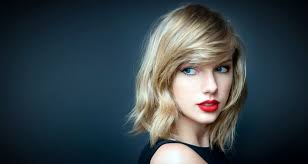
\includegraphics[width = \linewidth]{taylor.jpg}
 	\caption{input image for cartoonization 2}
 	\label{fig:inputCartoon2}
 \end{figure}
 
   \begin{figure}[h]
 	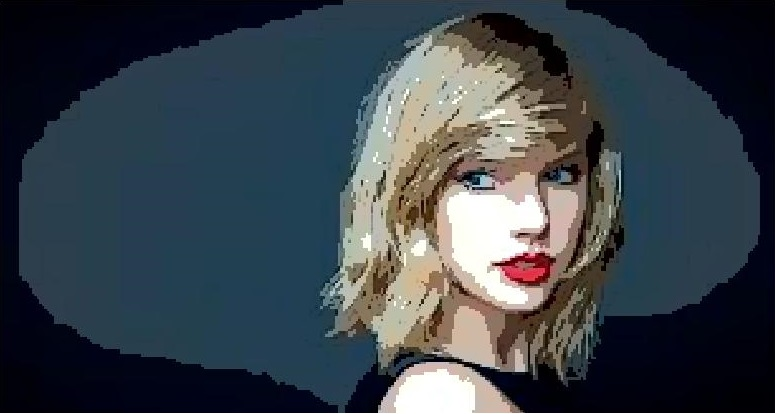
\includegraphics[width = \linewidth]{taylor_out.jpg}
 	\caption{output image for cartoonization 2}
 	\label{fig:outputCartoon2}
 \end{figure}
 

\begin{figure}[h]
 	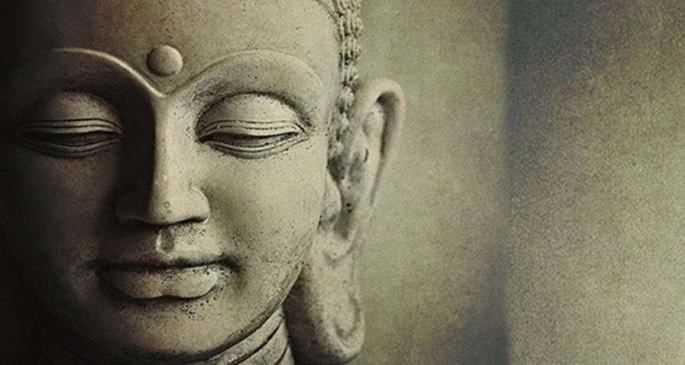
\includegraphics[width = \linewidth]{buddha.jpg}
 	\caption{input image for depth stylization}
 	\label{fig:inputDStylization}
 \end{figure}

 \begin{figure}[h]
 	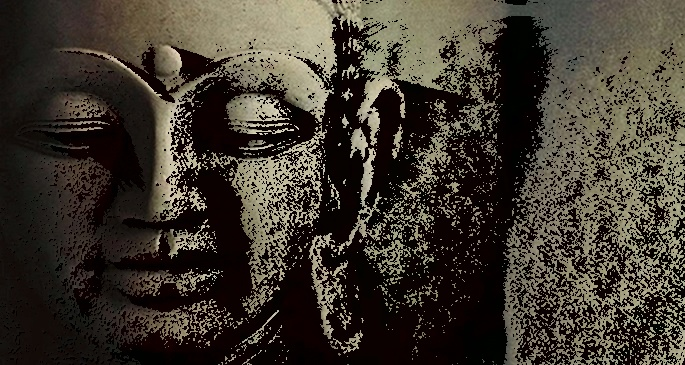
\includegraphics[width = \linewidth]{buddha_out2.jpg}
 	\caption{output for depth stylization}
 	\label{fig:outputDStylization}
 \end{figure} 
 
  \begin{figure}[h]
 	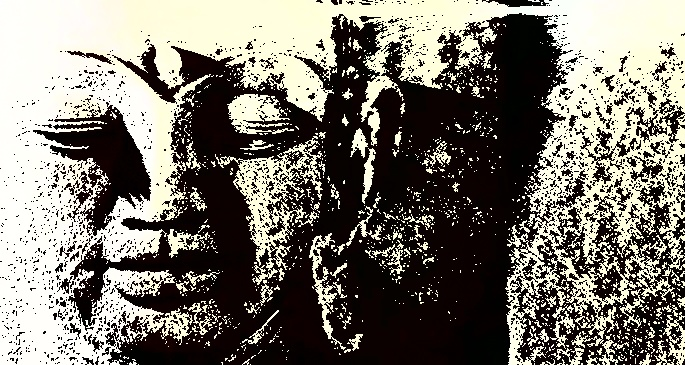
\includegraphics[width = \linewidth]{buddha_out_bw.jpg}
 	\caption{output for halftoning}
 	\label{fig:outputHalf}
 \end{figure} 
 
   \begin{figure}[h]
 	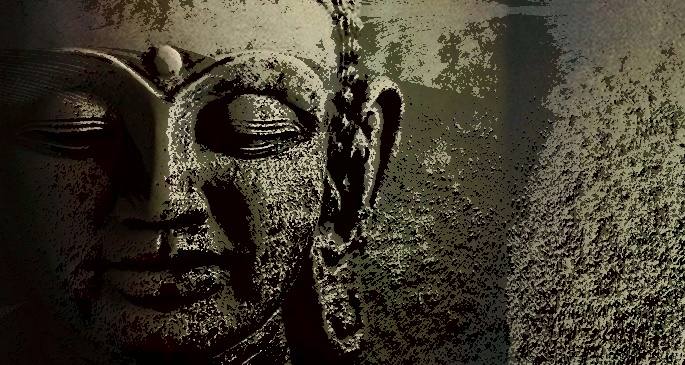
\includegraphics[width = \linewidth]{buddha_out_2sources.jpg}
 	\caption{output for multitoning}
 	\label{fig:outputMulti}
 \end{figure}
 
  \begin{figure}[h]
 	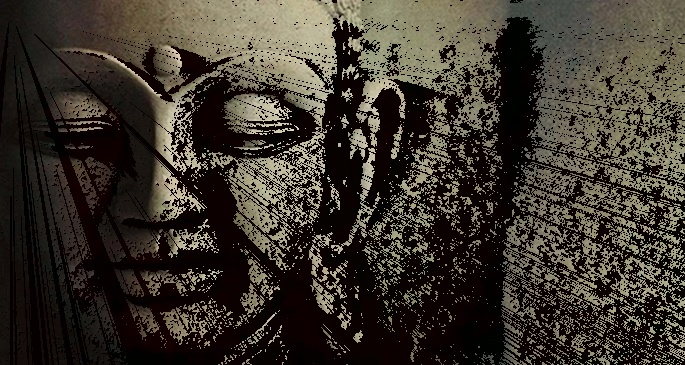
\includegraphics[width = \linewidth]{buddha_out_lines.jpg}
 	\caption{output for line effect}
 	\label{fig:outputLines}
 \end{figure} 


\section{Acknowledgement}
We would like to thank Professor Saumik Bhattacharya for their insightful lectures which helped alot for successful completion of the project. 

\begin{thebibliography}{9}
\bibitem{Domain} 
Domain Transform for Edge-Aware Image and Video Processing.
\textit{Eduardo S. L. Gastal, Manuel M. Oliveira.Instituto de Informatica – UFRGS}. 
 
\bibitem{einstein} 
Recursive Filtering in Image Processing 
\textit{Martin Vicanek}
 
\end{thebibliography}

\end{document}
